
%\section{Premilinaries}
\section{Background and Related Work}
\label{sec:background}
% \hjc{Combine this with related work + check if the topics discussed here are directly related to our contributions.}
%\hjc{Clean up required background + prelim + motivation are too much }


% \label{sec:goals}
This section includes the background and related works of \thename. Our work is primarily motivated by recent developments and the upcoming integrations of PIM architectures described in \ref{subsec:pim-bg}. Our work introduces a cooperation model for confidential computation that addresses the challenges of CPU-based enclaves (e.g., the lack of memory and side-channels). We explain the background for those challenges and the related work in~\ref{subsec:confidential}.



\subsection{Processing-In-Memory}
\label{subsec:pim-bg}
PIM is a general direction towards embedding processing capability inside memories to overcome the memory bandwidth bottleneck, as today's workload is becoming more and more data-intensive. We briefly explain the existing works on PIM from both the industry and academia.
%Then, we will explain the baseline PIM model, a generalized PIM architecture based on our observations, on which we build our architecture \thename.

\begin{figure}[b]
\centering
    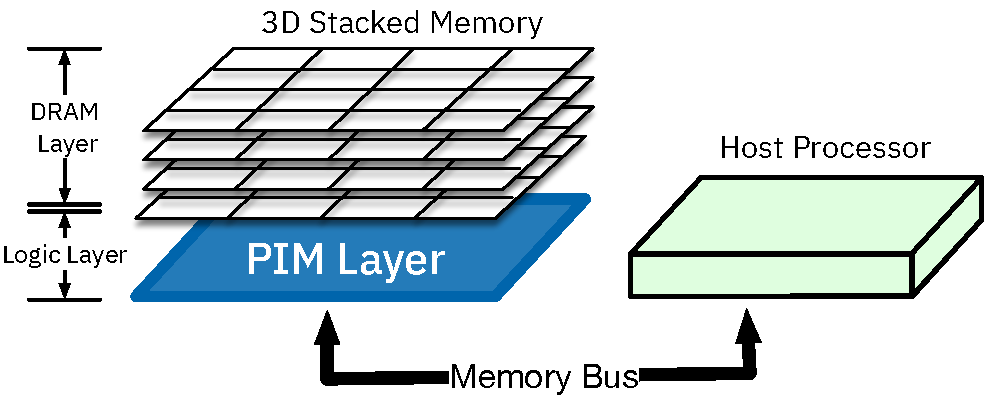
\includegraphics[width=0.80\columnwidth ]{figures/pim.pdf}
    \caption{Processing-In-Memory layer in 3D-stacked memory.}
    \label{fig:pim}
\end{figure}


\subsubsection{PIM hardware architectures.}
The progress made in 3D-stacked memory technology enabled embedding of logics or even processors into memory. Two of the most prominent example of 3D-stacked memory are \emph{Hybrid memory cube (HMC)}~\cite{hmc}, and \emph{High Bandwidth Memory (HBM)} \cite{amd-hbm,samsung-pim}. \autoref{fig:pim} demonstrates the architecture of 3D-stacked memory and the PIM layer. Stacked memory architectures vertically stack DRAM layers on top of each other and connect the vertical partitions of memory using high-bandwidth through-silicon vias (TSVs). A typical 3D-stacked memory configuration can employ thousands of TSVs \cite{primer-on-pim}, which makes its internal memory bandwidth far exceed that of traditional memory systems. At the bottom of the memory stacks, there is a \emph{PIM layer}, or logic layer, that can host hardware logic that can interact with both the host processor and the DRAM memory. The PIM layer can be special-purpose hardware logic~\cite{invisimem,prime} that is embedded into the memory chip, or a general-purpose processor~\cite{upmem,samsung-pim,smcsim,pim-architecture} that runs software called the \emph{PIM kernels}, analogous to the kernels loaded onto GPUs. Most 3D-stacked PIM architecture requires changes to the host-side processor~\cite{pim-architecture}, but PIM architectures that can integrate with commodity processors also exist~\cite{upmem,upmem-atc,pim-architecture}. UPMEM~\cite{upmem} introduced its PIM architecture on a traditional DRAM chip. Lee et al.~\cite{pim-architecture} designed and implemented a generalized PIM architecture and programming model to support PIM-accelerated DNN computation on HBM memory. Both of these prototypes have real hardware implementations and are compatible with off-the-shelf systems~\cite{upmem-atc,pim-architecture}.

%\hdr{Using PIM for security.} There have been works that harness PIM computation for security purposes. InvisiMem \cite{invisimem} and ObfusMem \cite{obfusmem} proposed enhancing the host-side memory controller and the memory-side memory controller with capabilities to form an encrypted communication channel that also encrypts the accessed address and type of operation (read or write). In doing so, the systems can provide security guarantees similar to Oblivious RAM (ORAM) without significant performance overhead~\cite{obfusmem,invisimem}. Other works demonstrated that PIM is beneficial for accelerating security operations \cite{sdimm, near-data-security, hega}. \cite{near-data-security} suggests delegating Bonsai Merkle Tree memory authentication operations to memory. Secure DIMM (SDIMM)~\cite{sdimm} offloads that a part of the ORAM access routine to logic inside a DIMM memory to reduce the bandwidth usage of ORAM algorithms. In \cite{hega}, the authors propose HEGA, a PIM architecture that accelerates homomorphic encryption search. All of those researches show that PIM can significantly reduce the memory bandwidth of memory-intensive security applications.
% \hdr{Acceleration of security operations.}




\newcommand{\goal}[1]{\hyperref[g#1]{O#1}}

\subsection{Confidential Computing in Cloud and Challenges}
\label{subsec:confidential}

Supporting confidential computing in the untrusted cloud is a common goal shared by the industry and academia, as evidenced by confidential computing services being offered by cloud service providers \cite{azure,google-confidential-computing,nitro}. 

% Several works have proposed various SGX-based confidential computation schemes. The works explored the design space in using Intel SGX for secure data computation in the cloud~\cite{vc3,enclavedb,occulemency}. VC3~\cite{vc3} proposes an architecture for performing distributed MapReduce in the untrusted cloud, in which sensitive code and data are protected. EnclaveDB~\cite{enclavedb} protects the database and the querying process using SGX. Occlumency~\cite{occulemency} proposes an SGX-based deep learning inference that ensures confidentiality and integrity of user data. 
\subsubsection{Secure enclaves and the cloud. }
Modern processor architectures support secure enclaves for isolated execution of sensitive code and data. Intel SGX~\cite{sgx} is the most commonly available secure enclave in the cloud. SGX provides protected memory pages called \emph{Enclave Page Cache (EPC)} in which the sensitive subset of a program and processed data can be protected. Memory accesses from the processor to the EPC region are automatically encrypted on the memory bus by the memory encryption engine~\cite{sgx-explained}. A remote user can verify the integrity of a deployed enclave through \emph{remote attestation}, a procedure that allows an enclave to \emph{attest} its code and data with a measurement, signed by a secure hardware cryptographic key. 

\subsubsection{Memory limitations of secure enclaves.} 
The limited memory capacity is one of the main factors that hinder the adoption of SGX-based secure enclaves. SGX has a limited EPC capacity of 128MB; large data computation has to be broken down into smaller batches~\cite{occulemency,bigmatrix}. DNN model-based inference frameworks that are aware of and optimized for the SGX's memory limitations are also proposed~\cite{occulemency,kim2020vessels}. Moreover, it is shown that EPC page swapping is expensive when a large amount of secure memory is used~\cite{zerotrace,scone} (up to $1000\times$ performance overhead). Designs for external secure storage devices for secure enclaves are also explored by several works to complement SGX's memory limitation~\cite{trustore,invisimem,obfusmem}.


\subsubsection{Side-channel attacks on enclaves.}
Researchers have shown that secure enclaves can fall vulnerable to side-channel attacks. The microarchitectural side-channels and the data access pattern captured on the memory bus are shown to be exploitable against SGX secure enclaves to undermine the confidentiality of the computed data~\cite{leaky-cauldron,sgx-cache-attack,sgx-grand-exposure,membuster}. Microarchitectural side-channel attacks exploit \emph{microarchitectural resources sharing} to extract sensitive information about the enclave execution~\cite{sgx-cache-attack,sgx-grand-exposure}. For instance, attackers can infer secret-dependent cache lines accesses of an enclave based on the cache timing~\cite{sgx-grand-exposure}. On the other hand, even though memory requests from an enclave are encrypted, the \emph{access pattern} of data can also leak secrets. Membuster~\cite{membuster} demonstrated an attack that uses a capturing device attached to the memory bus that extracts sensitive information only from the \emph{addresses side-channel} of SGX enclaves.

% \hdr{Approaches for side-channel elimination.} 
% The causes for most memory side-channels are the differences in the memory access pattern that depends on the secret input~\cite{raccoon}. Program obfuscation and oblivious RAM (ORAM) adaptations inside enclave~\cite{raccoon,zerotrace,obfuscuro} are the generally accepted solutions for memory side channels. Program obfuscation transforms potentially unsafe programs into side-channel-free programs~\cite{raccoon,obfuscuro,ghostrider}, while the use of ORAM algorithms hide the access pattern to sensitive data structures~\cite{raccoon,obfuscuro,zerotrace,ghostrider}. However, due to the high performance overhead, those approaches are often inapt for data-intensive computing.

% \new{
% Alternatively, there are also approaches that help eliminate side-channels from software, by providing ORAM-like obliviousness with trusted hardware~\cite{trustore,obfusmem,invisimem}. Obfusmem~\cite{obfusmem} and Invisimem~\cite{invisimem} construct a secure channel between the host CPU's memory controller and the memory-side memory controller to hide the memory access pattern. Trustore~\cite{trustore} uses a narrow single-channel to interface a PCIe storage and SGX enclave to mitigate side-channels in processor caches and address side-channel on the bus. }

\subsubsection{Extending trust to the peripheral devices.}
Since achieving trusted I/O with a device is not viable in SGX's security model, the device itself must actively participate in establishing a secure channel with the processor enclave. Existing works have presented peripheral device designs that create a secure communication channel with the host enclaves. Graviton~\cite{graviton} proposed a set of hardware modifications for GPUs that enables secure acceleration for confidential computing in the cloud. HIX~\cite{hix} sought to achieve the same goal but proposed modifications to the I/O interconnect between CPU and GPU. Trustore~\cite{trustore} uses an FPGA storage device to provide extra storage space that is free of memory side-channels for SGX. One design component these works have in common is remote attestation and secure communication channels. Our design, \thename, adapts many of the requirements for a device in extending processor enclave's trust to I/O devices generalized by the previous works.  

\subsection{Mitigations of Access Pattern Side-channels}
\label{subsec:oram}
Oblivious RAM (ORAM)~\cite{path-oram,ring-oram,freecursive-oram} is accepted as a general mitigation for the access pattern side-channels. ORAM algorithms transform the original data accesses into sequences of obfuscated accesses that seem random to attackers~\cite{ring-oram}. There have been adaptations of ORAM to SGX enclaves~\cite{zerotrace,obfuscuro} to hide the enclave's access patterns to sensitive data structures. Secure processor prototypes that integrate ORAM logic into the memory controller also exists~\cite{freecursive-oram,ascend} that hides the access pattern on the bus. However, the performance overhead of ORAM-based approaches may deter their adaption~\cite{zerotrace}. In response, alternative approaches are proposed that build an encrypted channel between the user and secure storage. Invisimem~\cite{invisimem} and Obfusmem~\cite{obfusmem} introduced encryption capabilities to the CPU-side and the memory-side controllers to encrypt the entire memory request, including the \emph{accessed address} and \emph{type of operation}, to achieve ORAM-like security guarantees. Trustore~\cite{trustore} employed the same technique to hide the address-based side-channel by establishing an encrypted channel between an SGX enclave and the secure FPGA-based storage. 
